\documentclass[border=3mm]{standalone}
\usepackage{tikz}
\usetikzlibrary{circuits.logic.US}

\begin{document}
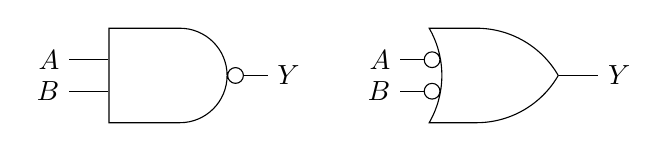
\begin{tikzpicture}[circuit logic US,
                    tiny circuit symbols,
                    every circuit symbol/.style={fill=white,draw,logic gate input sep=4mm, logic gate inverted radius=1mm}
]

\node [nand gate, inputs = nn] at (0,0) (nand1) {};
\node [or gate, inputs = ii, anchor=output] at ($(nand1.output)+(4.0cm,0)$) (or1) {};
%
\draw (nand1.input 1) -- ++(left:5mm) node[left] (B1) {$A$};
\draw (nand1.input 2) -- ++(left:5mm) node[left] (C1) {$B$};
\draw (nand1.output) -- ++(right:3mm) node[right] (Y1) {$Y$};

\draw (or1.input 1) -- ++(left:3mm) node[left] (B2) {$A$};
\draw (or1.input 2) -- ++(left:3mm) node[left] (C2) {$B$};
\draw (or1.output) -- ++(right:5mm) node[right] (Y2) {$Y$};
\end{tikzpicture}
\end{document}
